% Options for packages loaded elsewhere
% Options for packages loaded elsewhere
\PassOptionsToPackage{unicode}{hyperref}
\PassOptionsToPackage{hyphens}{url}
%
\documentclass[
  12pt,
  letterpaper,
  DIV=11,
  numbers=noendperiod]{scrreprt}
\usepackage{xcolor}
\usepackage[margin=1in]{geometry}
\usepackage{amsmath,amssymb}
\setcounter{secnumdepth}{5}
\usepackage{iftex}
\ifPDFTeX
  \usepackage[T1]{fontenc}
  \usepackage[utf8]{inputenc}
  \usepackage{textcomp} % provide euro and other symbols
\else % if luatex or xetex
  \usepackage{unicode-math} % this also loads fontspec
  \defaultfontfeatures{Scale=MatchLowercase}
  \defaultfontfeatures[\rmfamily]{Ligatures=TeX,Scale=1}
\fi
\usepackage{lmodern}
\ifPDFTeX\else
  % xetex/luatex font selection
\fi
% Use upquote if available, for straight quotes in verbatim environments
\IfFileExists{upquote.sty}{\usepackage{upquote}}{}
\IfFileExists{microtype.sty}{% use microtype if available
  \usepackage[]{microtype}
  \UseMicrotypeSet[protrusion]{basicmath} % disable protrusion for tt fonts
}{}
\usepackage{setspace}
\makeatletter
\@ifundefined{KOMAClassName}{% if non-KOMA class
  \IfFileExists{parskip.sty}{%
    \usepackage{parskip}
  }{% else
    \setlength{\parindent}{0pt}
    \setlength{\parskip}{6pt plus 2pt minus 1pt}}
}{% if KOMA class
  \KOMAoptions{parskip=half}}
\makeatother
% Make \paragraph and \subparagraph free-standing
\makeatletter
\ifx\paragraph\undefined\else
  \let\oldparagraph\paragraph
  \renewcommand{\paragraph}{
    \@ifstar
      \xxxParagraphStar
      \xxxParagraphNoStar
  }
  \newcommand{\xxxParagraphStar}[1]{\oldparagraph*{#1}\mbox{}}
  \newcommand{\xxxParagraphNoStar}[1]{\oldparagraph{#1}\mbox{}}
\fi
\ifx\subparagraph\undefined\else
  \let\oldsubparagraph\subparagraph
  \renewcommand{\subparagraph}{
    \@ifstar
      \xxxSubParagraphStar
      \xxxSubParagraphNoStar
  }
  \newcommand{\xxxSubParagraphStar}[1]{\oldsubparagraph*{#1}\mbox{}}
  \newcommand{\xxxSubParagraphNoStar}[1]{\oldsubparagraph{#1}\mbox{}}
\fi
\makeatother


\usepackage{longtable,booktabs,array}
\newcounter{none} % for unnumbered tables
\usepackage{calc} % for calculating minipage widths
% Correct order of tables after \paragraph or \subparagraph
\usepackage{etoolbox}
\makeatletter
\patchcmd\longtable{\par}{\if@noskipsec\mbox{}\fi\par}{}{}
\makeatother
% Allow footnotes in longtable head/foot
\IfFileExists{footnotehyper.sty}{\usepackage{footnotehyper}}{\usepackage{footnote}}
\makesavenoteenv{longtable}
\usepackage{graphicx}
\makeatletter
\newsavebox\pandoc@box
\newcommand*\pandocbounded[1]{% scales image to fit in text height/width
  \sbox\pandoc@box{#1}%
  \Gscale@div\@tempa{\textheight}{\dimexpr\ht\pandoc@box+\dp\pandoc@box\relax}%
  \Gscale@div\@tempb{\linewidth}{\wd\pandoc@box}%
  \ifdim\@tempb\p@<\@tempa\p@\let\@tempa\@tempb\fi% select the smaller of both
  \ifdim\@tempa\p@<\p@\scalebox{\@tempa}{\usebox\pandoc@box}%
  \else\usebox{\pandoc@box}%
  \fi%
}
% Set default figure placement to htbp
\def\fps@figure{htbp}
\makeatother


% definitions for citeproc citations
\NewDocumentCommand\citeproctext{}{}
\NewDocumentCommand\citeproc{mm}{%
  \begingroup\def\citeproctext{#2}\cite{#1}\endgroup}
\makeatletter
 % allow citations to break across lines
 \let\@cite@ofmt\@firstofone
 % avoid brackets around text for \cite:
 \def\@biblabel#1{}
 \def\@cite#1#2{{#1\if@tempswa , #2\fi}}
\makeatother
\newlength{\cslhangindent}
\setlength{\cslhangindent}{1.5em}
\newlength{\csllabelwidth}
\setlength{\csllabelwidth}{3em}
\newenvironment{CSLReferences}[2] % #1 hanging-indent, #2 entry-spacing
 {\begin{list}{}{%
  \setlength{\itemindent}{0pt}
  \setlength{\leftmargin}{0pt}
  \setlength{\parsep}{0pt}
  % turn on hanging indent if param 1 is 1
  \ifodd #1
   \setlength{\leftmargin}{\cslhangindent}
   \setlength{\itemindent}{-1\cslhangindent}
  \fi
  % set entry spacing
  \setlength{\itemsep}{#2\baselineskip}}}
 {\end{list}}
\usepackage{calc}
\newcommand{\CSLBlock}[1]{\hfill\break\parbox[t]{\linewidth}{\strut\ignorespaces#1\strut}}
\newcommand{\CSLLeftMargin}[1]{\parbox[t]{\csllabelwidth}{\strut#1\strut}}
\newcommand{\CSLRightInline}[1]{\parbox[t]{\linewidth - \csllabelwidth}{\strut#1\strut}}
\newcommand{\CSLIndent}[1]{\hspace{\cslhangindent}#1}



\setlength{\emergencystretch}{3em} % prevent overfull lines

\providecommand{\tightlist}{%
  \setlength{\itemsep}{0pt}\setlength{\parskip}{0pt}}



 


\KOMAoption{captions}{tableheading}
\usepackage{chngcntr}
\counterwithout{equation}{chapter}
\counterwithout{footnote}{chapter}
\setkomafont{disposition}{\normalfont\bfseries}
\setlength{\emergencystretch}{3em}
\makeatletter
\@ifpackageloaded{caption}{}{\usepackage{caption}}
\AtBeginDocument{%
\ifdefined\contentsname
  \renewcommand*\contentsname{Table of contents}
\else
  \newcommand\contentsname{Table of contents}
\fi
\ifdefined\listfigurename
  \renewcommand*\listfigurename{List of Figures}
\else
  \newcommand\listfigurename{List of Figures}
\fi
\ifdefined\listtablename
  \renewcommand*\listtablename{List of Tables}
\else
  \newcommand\listtablename{List of Tables}
\fi
\ifdefined\figurename
  \renewcommand*\figurename{Figure}
\else
  \newcommand\figurename{Figure}
\fi
\ifdefined\tablename
  \renewcommand*\tablename{Table}
\else
  \newcommand\tablename{Table}
\fi
}
\@ifpackageloaded{float}{}{\usepackage{float}}
\floatstyle{ruled}
\@ifundefined{c@chapter}{\newfloat{codelisting}{h}{lop}}{\newfloat{codelisting}{h}{lop}[chapter]}
\floatname{codelisting}{Listing}
\newcommand*\listoflistings{\listof{codelisting}{List of Listings}}
\makeatother
\makeatletter
\makeatother
\makeatletter
\@ifpackageloaded{caption}{}{\usepackage{caption}}
\@ifpackageloaded{subcaption}{}{\usepackage{subcaption}}
\makeatother
\usepackage{bookmark}
\IfFileExists{xurl.sty}{\usepackage{xurl}}{} % add URL line breaks if available
\urlstyle{same}
% fallback for those not using the hyperref driver hyperxmp:
\makeatletter
\@ifundefined{xmpquote}{\newcommand{\xmpquote}[1]{#1}}{}
\makeatother
\hypersetup{
  hidelinks,
  pdfcreator={LaTeX via pandoc}}


\author{}
\date{}
\begin{document}


\setstretch{1.2}
\begin{titlepage}
\centering
\vspace*{1cm}
{\Large\bfseries Probabilistic Forecasting of Canadian Government Yields:\par}
\vspace{0.4cm}
{\Large\bfseries A Bayesian Stochastic-Volatility Extension of Dynamic Nelson--Siegel\par}
\vspace{1.6cm}
{\large Author: Ethan [full name to be confirmed]\par}
\vspace{0.7cm}
October 2026\par
\vspace{0.7cm}
Supervisor(s): [to be confirmed]\par
\vfill
A project\par
In partial fulfilment of the requirement for\par
Master of Quantitative Finance\par
University of Waterloo\par
\vspace{1cm}
\textbf{INTERNAL FIRST DRAFT -- SCIENTIFICALLY INCOMPLETE}\par
Not for submission: supervisor approval of AI use and validation of the Bayesian comparison remain outstanding.
\end{titlepage}
\pagenumbering{roman}
\chapter*{Abstract}
\addcontentsline{toc}{chapter}{Abstract}

This study investigates whether stochastic factor volatility improves
probabilistic forecasts of Canadian government yields within a two-step
Dynamic Nelson--Siegel framework. The proposed experiment compares six
models at one- and four-week horizons, using eight zero-coupon
maturities, an initial 2000--2015 estimation window and expanding-window
forecasts over 2016--2025. A completed six-model computation produced
1,560 forecast records at 130 origins, but subsequent verification
identified implementation defects and severe stochastic-volatility chain
non-convergence. Those outputs are quarantined and do not establish an
advantage for Bayesian stochastic volatility. A separately tested rerun
of three classical benchmarks produced 780 forecast records with
analytic predictive moments. At four weeks, the random walk attained a
mean Dawid--Sebastiani score of −36.006, compared with −24.394 for
PCA--VAR and −21.453 for two-step Nelson--Siegel. Its pooled yield RMSE
was 0.213 percentage points and its pooled marginal 90\% interval
coverage was 87.1\%. These findings are descriptive results for a
historical data vintage, not real-time implementable forecasts: the
public yield-curve series has a publication lag. This partial first
draft preserves the approved Bayesian research question, documents the
failed inference, and provides reproducible classical results. The
primary constant-volatility versus stochastic-volatility Bayesian
comparison remains unresolved.

\clearpage
\chapter*{Acknowledgements and research disclosure}
\addcontentsline{toc}{chapter}{Acknowledgements and research disclosure}

This internal draft was prepared with AI assistance for literature
retrieval, programming, computational auditing and writing. The student
must review the code, understand the methods, independently assess all
scientific claims and discuss the permitted use of AI with the
supervisor before using this material for the research paper. The MQF
guidelines explicitly require prior discussion of AI use; that approval
has not been established in the project materials. This disclosure does
not substitute for approval.

The Bank of Canada is acknowledged as the source of the Canadian
zero-coupon yield-curve data. No endorsement by the Bank is implied.
Source access and bibliographic verification are distinguished from
complete-paper review in the accompanying literature inventory. The
originally supplied proposal, guidelines and raw data have been
retained. No submission or communication with the university has been
made.

The draft is deliberately incomplete where the evidence is incomplete.
In particular, a successful numerical process exit is not evidence of
correct Bayesian inference. Results from the failed
stochastic-volatility computation are retained for diagnosis but are not
presented as empirical findings supporting the hypothesis. The validated
tables are generated from a separate classical-benchmark run.

\clearpage
\tableofcontents
\clearpage
\listoftables
\clearpage
\listoffigures
\clearpage
\pagenumbering{arabic}

\chapter{Introduction}\label{sec-introduction}

\section{Motivation and research
problem}\label{motivation-and-research-problem}

A government yield curve relates the interest rate on a zero-coupon
claim to the time remaining until its payment. A short-maturity rate and
a long-maturity rate need not move together. Consequently, a single
forecast of a policy rate or a ten-year yield is not a forecast of the
entire curve. Fixed-income risk management requires scenarios describing
both the size of yield movements and the way movements at different
maturities occur together.

The Dynamic Nelson--Siegel (DNS) representation compresses the curve
into three factors with level, slope and curvature loading patterns.
This provides a parsimonious starting point for forecasting and an
interpretable alternative to a high-dimensional unrestricted yield
model. The approved proposal builds on the dynamic forecasting framework
of Diebold \& Li (\citeproc{ref-diebold2006forecasting}{2006}) and the
Bayesian stochastic-volatility literature represented by Hautsch \& Yang
(\citeproc{ref-hautsch2012bayesian}{2012}).

The central research question is unchanged from the proposal:
\textbf{does incorporating Bayesian stochastic volatility into DNS
factor dynamics improve out-of-sample probabilistic forecasts of
Canadian government yields relative to constant-volatility DNS models
and standard forecasting benchmarks?} The question concerns predictive
uncertainty, not merely whether fitted curves closely reproduce observed
yields. A model can have a small cross-sectional reconstruction error
and still produce a poorly calibrated distribution for future curves.

A useful distinction is between a point forecast and a predictive
distribution. The first summarizes a future curve by its conditional
mean. The second assigns probabilities to alternative future curves. Two
models can have similar conditional means yet differ materially in
forecast variances, interval widths and cross-maturity dependence. The
proposal therefore makes a mean--covariance score the primary criterion
and supplements it with an ensemble-based distributional score.

\section{Intended contribution and scope of this
draft}\label{intended-contribution-and-scope-of-this-draft}

The intended contribution is a controlled comparison between Bayesian
DNS models with constant and stochastic factor volatility. Both are to
use identical extracted factors, stationary univariate AR(1) mean
equations, reconstruction-error treatment and forecast dates. The
stochastic-volatility specification adds latent time-varying factor
variances. Conventional models provide external competitiveness checks
rather than single-change causal comparisons.

The present draft does not claim that this contribution has been
demonstrated. The original six-model run completed, but an independent
mathematical and diagnostic audit found defects. Those defects affect
the interpretation of its scores even though the saved arrays are
finite. Reproducing an incorrect calculation cannot turn it into a valid
scientific result. Accordingly, this paper reports a separately verified
classical baseline experiment and documents why the primary Bayesian
inference is not accepted.

This distinction is important for interpreting negative results. Failure
of an estimation implementation is not evidence against stochastic
volatility. Conversely, favorable scores from an unconverged sampler are
not evidence for it. The appropriate conclusion is narrower: the
completed computation does not resolve the research question, while the
validated baseline results establish the standard that a corrected
Bayesian model must meet.

\section{Organization}\label{organization}

Section~\ref{sec-literature} connects the model and evaluation choices
to the literature. Section~\ref{sec-data} documents provenance, units
and forecast-date construction. Section~\ref{sec-methods} gives the
complete proposed model ladder. Section~\ref{sec-design} defines
evaluation and scientific acceptance criteria. Section~\ref{sec-results}
presents accepted classical results and contrasts them with the
quarantined computation. Section~\ref{sec-risk} gives a restricted
scenario-risk illustration. Section~\ref{sec-conclusions} states the
defensible conclusions and unfinished work. Appendices derive forecast
equations and record numerical verification.

\chapter{Literature and conceptual framework}\label{sec-literature}

\section{Representation versus
dynamics}\label{representation-versus-dynamics}

The proposal uses the Nelson--Siegel cross-section as a representation
of yield-curve shape and AR dynamics as a law of motion for its factors.
These are separate modeling choices. Re-estimating a curve at each
observation produces a sequence of factors, but a forecast additionally
requires a probability model for their future values. Diebold \& Li
(\citeproc{ref-diebold2006forecasting}{2006}) provides the central
forecasting reference; Diebold et al.
(\citeproc{ref-diebold2006macroeconomy}{2006}) provides a related
dynamic latent-factor treatment linking yields and the macroeconomy.

The interpretation of the three factors follows from their loadings, not
from a claim that all factors are stationary or cointegrated. In the
convention used here, the level loading is one at every maturity. The
slope loading is positive at short maturities and tends toward zero at
long maturities. Curvature has a hump-shaped loading. Claims about
integration orders or economic identification require further testing
and are not inferred from the labels.

A PCA factor model is a useful external comparison because its basis is
selected from yield variation rather than prescribed by a parametric
maturity function. Its factors do not generally have the same economic
interpretation as DNS factors. A favorable comparison between DNS and
PCA could reflect representation, mean dynamics, residual covariance or
estimation uncertainty. It cannot isolate volatility dynamics in the way
the planned Bayesian pair can.

\section{Stochastic volatility and the controlled
comparison}\label{stochastic-volatility-and-the-controlled-comparison}

Hautsch \& Yang (\citeproc{ref-hautsch2012bayesian}{2012}) and Caldeira
et al. (\citeproc{ref-caldeira2010bayesian}{2010}) are verified
bibliographic references on Bayesian Nelson--Siegel models with
stochastic volatility. Their relevance is to the modeling possibility,
not a guarantee of forecasting improvement in Canada. The specification
in the proposal is deliberately a two-step approximation: extracted
factors are treated as observations when fitting their second-stage
dynamics. It must not be described as equivalent to a unified
latent-factor state-space model.

Omori et al. (\citeproc{ref-omori2007stochastic}{2007}) is the
methodological reference for efficient stochastic-volatility inference
using a mixture approximation. The no-leverage model in the proposal is
a restriction relative to the leverage setting named in that article. A
valid implementation requires the actual approximation coefficients,
parameter conventions and full conditional distributions to agree.
Merely citing the article does not validate a transcribed table or a
custom Gibbs sampler.

The proposal also identifies Sarkisian
(\citeproc{ref-sarkisian2024bayesian}{2024}) as a related Master's
thesis. Its institutional provenance is distinct from the countries or
instruments used empirically. This draft does not infer a Dutch-yield
sample from the university's location. Detailed thesis findings and
comparisons to this project are contingent on the access evidence
recorded in \texttt{docs/literature\_inventory.md}.

\section{What proper scoring rules
establish}\label{what-proper-scoring-rules-establish}

The literature on proper scoring rules motivates evaluation of
predictive distributions rather than exclusively point errors
(\citeproc{ref-gneiting2007strictly}{Gneiting \& Raftery, 2007}). A
scoring rule is proper when the expected score is optimized by reporting
the relevant true predictive object. Propriety does not eliminate
sampling variability, dependence among verification dates, approximation
error in simulated ensembles, or errors in the model implementation.

The Dawid--Sebastiani score (DSS) uses a predictive mean and covariance.
Its scoring-rule foundation is related to Dawid \& Sebastiani
(\citeproc{ref-dawid1999coherent}{1999}). In the present multivariate
form it cannot distinguish two distributions that share the same mean
and covariance. It therefore must not be called a strictly
discriminating test of the entire posterior-predictive distribution. An
Energy Score provides complementary information about simulated yield
vectors, while the Variogram Score emphasizes pairwise cross-maturity
contrasts (\citeproc{ref-scheuerer2015variogram}{Scheuerer \& Hamill,
2015}).

Patton (\citeproc{ref-patton2011volatility}{2011}) studies comparison
using imperfect volatility proxies. It is relevant motivation for
thinking carefully about variance losses, but it does not itself
establish robustness of every eight-dimensional covariance score used
with estimated zero-coupon curves. The observed yield vector here is the
forecast target; it is not a direct observation of a latent conditional
covariance matrix.

\section{Comparison uncertainty and evidence
limits}\label{comparison-uncertainty-and-evidence-limits}

Hansen et al. (\citeproc{ref-hansen2011model}{2011}) introduces the
Model Confidence Set (MCS). The concept is useful when the data cannot
sharply distinguish forecasts. Correct implementation requires a
documented equal-predictive-ability statistic, an appropriate
elimination rule and resampling that respects loss dependence. A set
generated by an arbitrary elimination routine is not validated merely by
using the MCS name.

This draft distinguishes verified bibliography metadata from verified
paper contents. Crossref responses are cached for the journal articles.
Access to publisher abstracts does not count as complete-paper review.
Where complete texts remain unavailable, detailed empirical assertions
have been omitted rather than reconstructed from titles or secondary
descriptions. The literature inventory records remaining access gaps and
any full-text evidence obtained.

\chapter{Data and information sets}\label{sec-data}

\section{Source and provenance}\label{source-and-provenance}

The primary source is the Bank of Canada's public zero-coupon
yield-curve series (\citeproc{ref-bocdata}{Bank of Canada, 2026}). Its
source page describes daily curves derived from Government of Canada
bonds and treasury bills, a quarterly maturity grid from 0.25 through 30
years, decimal yield units, missing observations marked \texttt{na}, and
a typical two-week update lag. These are estimated curves rather than a
panel of directly traded zero-coupon security prices at all maturities.
The Bank identifies Bolder et al.
(\citeproc{ref-bolder2004canadian}{2004}) as the methodology reference.

The project originally contained a raw Canadian CSV. Its original
retrieval transaction is not authenticated; a filesystem modification
timestamp is not a server download receipt. This limitation is explicit
in the manifest. A fresh non-destructive check downloaded December 2015
observations from the official endpoint. The eight selected maturities
matched the supplied file exactly on 21 complete dates. This is a
source-consistency check for that slice, not proof that every historical
row has been independently re-downloaded or that a vintage is unrevised.

The raw file is preserved separately from the processed weekly panel.
The canonical processor is \texttt{src/prepare\_data.py}; the
source-check script is \texttt{src/source\_data\_check.py}. Source URLs,
retrieval timestamps, checksums and the slice comparison are stored
under \texttt{docs/sources/}. Previously supplied U.S. data are retained
but are not part of the approved Canadian forecasting experiment.

\section{Cleaning, units and weekly
sampling}\label{cleaning-units-and-weekly-sampling}

The selected maturity grid is \((0.25,0.5,1,2,5,7,10,30)\) years.
Headers are stripped of leading spaces; dates are parsed and checked for
uniqueness. A daily observation is eligible only if all eight selected
yields are present. The processor converts decimal yields to percentage
points by multiplying by 100 and selects the last eligible observation
in each ISO calendar week. This is neither averaging nor interpolation.

The raw Canadian file contains 6,974 daily rows, of which 335 do not
supply a complete selected curve. The remaining 6,639 complete rows
produce 1,396 weekly observations. These counts refer to the complete
supplied file, not the restricted research sample. An earlier diagnostic
message incorrectly said zero missing rows were dropped; the canonical
manifest corrects that statement.

The research sample excludes the weekly observation dated 31 December
1999 and all dates in 2026. It contains 1,356 weekly observations: 835
through the end of 2015 and 521 in 2016--2025. Table~\ref{tbl-data}
summarizes this restricted sample. All scores use percentage-point
units; hence 0.01 percentage points equals one basis point. Comparisons
use identical units across models. Changing units shifts
determinant-based scores and rescales distance-based scores.

\begin{longtable}[]{@{}lllll@{}}
\caption{Weekly Canadian yields, 2000--2025, in percentage
points.}\label{tbl-data}\tabularnewline
\toprule\noalign{}
Maturity & Mean & SD & Min & Max \\
\midrule\noalign{}
\endfirsthead
\toprule\noalign{}
Maturity & Mean & SD & Min & Max \\
\midrule\noalign{}
\endhead
\bottomrule\noalign{}
\endlastfoot
0.250 & 2.109 & 1.612 & 0.049 & 5.756 \\
0.500 & 2.166 & 1.594 & 0.093 & 5.951 \\
1.000 & 2.261 & 1.568 & 0.123 & 6.166 \\
2.000 & 2.367 & 1.491 & 0.144 & 6.401 \\
5.000 & 2.733 & 1.451 & 0.294 & 6.484 \\
7.000 & 2.940 & 1.446 & 0.354 & 6.524 \\
10.000 & 3.179 & 1.404 & 0.482 & 6.556 \\
30.000 & 3.438 & 1.226 & 0.968 & 5.976 \\
\end{longtable}

\begin{figure}

\centering{

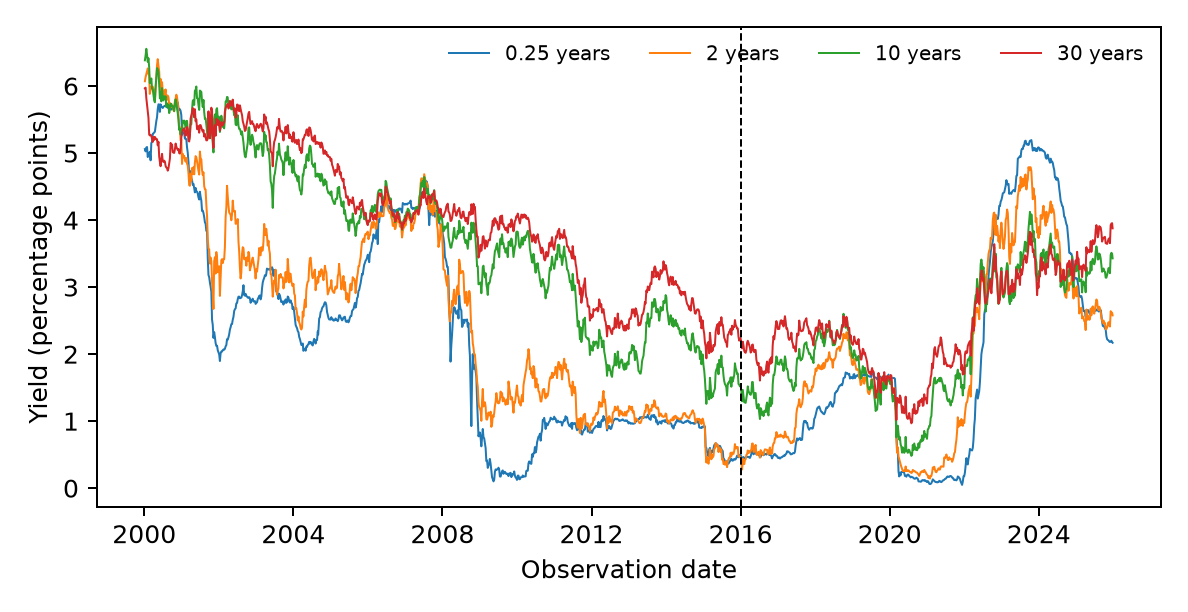
\includegraphics[width=0.95\linewidth,height=\textheight,keepaspectratio]{../figures/validated/yield_history.png}

}

\caption{\label{fig-history}Selected Canadian yield histories. The
vertical line marks the start of the evaluation period; observations are
not assumed publicly available contemporaneously.}

\end{figure}%

\section{Forecast dates and calendar
interpretation}\label{forecast-dates-and-calendar-interpretation}

Forecast horizons count weekly observations, not a fixed number of
trading days. Every fourth weekly observation in the out-of-sample
period is considered as an origin. An origin is retained only if both
its one- and four-observation-ahead targets lie in 2016--2025. This
gives 130 common origins, from 8 January 2016 to 28 November 2025. The
otherwise candidate observation near the end of December 2025 is
excluded because its four-week target is outside the sample.

Holidays can change the weekday and the number of elapsed calendar days
without changing the weekly index horizon. The origin-audit CSV records
origin and target dates, training counts and elapsed days. The sample
contains no gap exceeding ten calendar days between successive weekly
observations. A forecast labeled four weeks should therefore be read as
four weekly sampling steps, with the exact target date supplied in the
audit.

\section{Observation-time versus publication-time
information}\label{observation-time-versus-publication-time-information}

The experiments fit models only to observations dated no later than the
origin. Lambda selection also uses only the initial training sample.
This prevents future-dated observation leakage within the supplied
historical panel. It does \textbf{not} establish a real-time forecasting
design.

The Bank's typical two-week publication lag means a curve with
observation date \(t\) would not normally be publicly available to an
investor at \(t\). In addition, the supplied panel is a later historical
vintage. These experiments are therefore \textbf{retrospective
observation-time forecasts}, not operational forecasts under the public
release-time information set. A genuine release-time backtest needs
dated releases or a conservative availability-lag rule, with forecast
targets and information sets redesigned explicitly. A fixed lag alone
cannot eliminate uncertainty about historical revisions.

This is a substantive deviation from a strict interpretation of
``information available at the forecast origin.'' The observation-date
experiment is retained to preserve the proposal's principal design, but
the real-time implementation claim is withdrawn. No result in this draft
should be interpreted as executable performance at historical trading
dates.

\chapter{Model specifications}\label{sec-methods}

\section{Nelson--Siegel observation
equation}\label{nelsonsiegel-observation-equation}

Let \(Y_t\) be the eight-dimensional yield vector and
\(f_t=(L_t,S_t,C_t)'\) the factors. For maturity \(\tau\) in years
define

\begin{equation}\protect\phantomsection\label{eq-loadings}{
s(\tau;\lambda)=\frac{1-e^{-\lambda\tau}}{\lambda\tau},
\qquad c(\tau;\lambda)=s(\tau;\lambda)-e^{-\lambda\tau}.
}\end{equation}

The row of the loading matrix at \(\tau\) is \((1,s,c)\). This fixes the
slope sign convention consistently across equations and code. The
observation equation is

\begin{equation}\protect\phantomsection\label{eq-observation}{
Y_t=\Lambda(\lambda)f_t+\varepsilon_t,
\qquad \varepsilon_t\sim N(0,R_t).
}\end{equation}

The decay rate has units of inverse years; it is not a monthly
autoregressive parameter. Grid search over 160 values from 0.05 through
2.0 inverse years minimizes initial-window cross-sectional squared
errors. The selected value is 0.516038 inverse years and is fixed
thereafter. This selection uses the initial window only; sensitivity to
the grid and alternative selection losses remains future robustness
work.

At each date the two-step factor estimator is

\begin{equation}\protect\phantomsection\label{eq-extraction}{
\widehat f_t=(\Lambda'\Lambda)^{-1}\Lambda'Y_t.
}\end{equation}

The implementation uses least squares rather than explicitly forming
this inverse. Reconstruction variance at each maturity is the
origin-specific mean squared reconstruction error, floored at
\(10^{-6}\) squared percentage points. The diagonal \(R_t\) is a
modeling approximation, not a proof that residual errors are
independent. Small residual eigenvalues can materially affect an
eight-dimensional score.

\section{Complete benchmark ladder and acceptance
status}\label{complete-benchmark-ladder-and-acceptance-status}

\begin{longtable}[]{@{}
  >{\raggedright\arraybackslash}p{(\linewidth - 4\tabcolsep) * \real{0.3333}}
  >{\raggedright\arraybackslash}p{(\linewidth - 4\tabcolsep) * \real{0.3333}}
  >{\raggedright\arraybackslash}p{(\linewidth - 4\tabcolsep) * \real{0.3333}}@{}}
\caption{The complete proposal ladder. Non-acceptance is not a silent
omission.}\label{tbl-ladder}\tabularnewline
\toprule\noalign{}
\begin{minipage}[b]{\linewidth}\raggedright
Model
\end{minipage} & \begin{minipage}[b]{\linewidth}\raggedright
Proposed specification
\end{minipage} & \begin{minipage}[b]{\linewidth}\raggedright
Status in this draft
\end{minipage} \\
\midrule\noalign{}
\endfirsthead
\toprule\noalign{}
\begin{minipage}[b]{\linewidth}\raggedright
Model
\end{minipage} & \begin{minipage}[b]{\linewidth}\raggedright
Proposed specification
\end{minipage} & \begin{minipage}[b]{\linewidth}\raggedright
Status in this draft
\end{minipage} \\
\midrule\noalign{}
\endhead
\bottomrule\noalign{}
\endlastfoot
M0 & Yield random walk; Gaussian historical-change covariance &
Independently rerun and reported \\
M1 & Three PCA factors with VAR(1), plus reconstruction noise &
Independently rerun and reported \\
M2 & Two-step DNS; independent Gaussian AR(1) factors & Independently
rerun and reported \\
M3 & Gaussian DNS state-space; Kalman filter and likelihood estimation &
Executed; results not accepted \\
M4 & Bayesian two-step DNS with constant volatility & Executed with
deviations; not accepted \\
M5 & Bayesian two-step DNS with stochastic factor volatility & Failed
inference audit; quarantined \\
\end{longtable}

\section{Random-walk and PCA--VAR
forecasts}\label{random-walk-and-pcavar-forecasts}

M0 sets the future mean equal to the current curve. For horizon \(h\),
its covariance is the sample covariance of overlapping historical
\(h\)-step yield changes within the expanding window. This is a
zero-drift mean specification; estimating a change covariance does not
insert the historical mean change into the forecast. Covariance
eigenvalues are floored using the fixed training-only numerical rule.

M1 centers the expanding yield panel, estimates its first three
principal components and fits a VAR(1) with an intercept to their
scores. If the score equation is \(g_{t+1}=d+Ag_t+v_{t+1}\) with
innovation covariance \(Q\), the recursive forecast is

\begin{equation}\protect\phantomsection\label{eq-var-forecast}{
m_{k+1}=d+Am_k,\qquad V_{k+1}=AV_kA'+Q,
\quad m_0=g_t,\ V_0=0.
}\end{equation}

The yield mean adds the training center to the basis-projected score
mean. The covariance adds diagonal cross-sectional reconstruction error
to the projected score uncertainty. The PCA basis and VAR are refitted
at every origin, never estimated on the full sample. Finite-horizon
forecasts are computed directly; the validated classical runner does not
silently impose stationary coefficient clipping.

\section{Two-step Gaussian DNS}\label{two-step-gaussian-dns}

M2 fits a separate Gaussian AR(1) mean equation to each extracted
factor:

\begin{equation}\protect\phantomsection\label{eq-ar}{
f_{j,t+1}=a_j+b_j f_{j,t}+\eta_{j,t+1},
\quad \eta_{j,t+1}\sim N(0,q_j).
}\end{equation}

For the classical benchmark the fitted intercept and slope are
unrestricted least-squares estimates. Conditional on fitted parameters,
factor forecast moments are

\begin{equation}\protect\phantomsection\label{eq-ar-moments}{
 m_{j,h}=b_j^h f_{j,t}+a_j\sum_{k=0}^{h-1}b_j^k,
\qquad v_{j,h}=q_j\sum_{k=0}^{h-1}b_j^{2k}.
}\end{equation}

The yield covariance is \(\Lambda\operatorname{diag}(v_h)\Lambda'+R_t\).
Parameter uncertainty is not added to this classical plug-in forecast.
Factor innovation independence is an explicit restriction; PCA--VAR has
a full three-dimensional innovation covariance instead. Thus M1 and M2
differ in more than their cross-sectional basis.

\section{Gaussian latent-state DNS}\label{gaussian-latent-state-dns}

M3 estimates factors jointly through a Gaussian observation equation and
state transition. The executed version restricts transition and process
covariance to be diagonal and separately estimates diagonal measurement
covariance. Kalman filtering provides the filtered state and covariance;
likelihood maximization estimates parameters.

For transition matrix \(A\), filtered covariance \(P_t\) and process
covariance \(Q\), the horizon covariance must be

\begin{equation}\protect\phantomsection\label{eq-kalmanforecast}{
P_{t+h|t}=A^hP_t(A^h)'+\sum_{k=0}^{h-1}A^kQ(A^k)'.
}\end{equation}

The original implementation applied squared transition powers on each
side of \(P_t\), incorrectly attenuating its contribution. A regression
test against Equation~\ref{eq-kalmanforecast} exposed the defect and the
equation in code was corrected. The prior run's optimizer reported
success at all 130 origins, but optimizer success cannot repair a
forecast-covariance error or prove global likelihood maximization. A
corrected M3 rerun, additional start-value checks and independent
state-space validation remain outstanding.

\section{Bayesian constant-volatility
DNS}\label{bayesian-constant-volatility-dns}

The intended M4 uses the same factor AR(1) mean equation as M5,
stationary \(b_j\), fixed prior specifications and posterior-predictive
simulation at each origin. The original execution instead drew directly
from a truncated conjugate normal--inverse-gamma posterior. Independent
exact posterior draws can be useful, but this is a deviation from the
proposal's rolling MCMC requirement and must be stated rather than
described as MCMC.

More importantly, its coefficient prior scaled with the innovation
variance, while M5 used an unscaled coefficient prior. Consequently, the
pair did not isolate only volatility dynamics. Their predictive scores
cannot be interpreted as a controlled test of the primary hypothesis. A
revised pair must match the AR coefficient priors and explain how the
constant variance prior relates to the stochastic-volatility prior.
These specifications must be fixed without evaluating alternative
choices on out-of-sample scores.

\section{Bayesian stochastic-volatility
DNS}\label{bayesian-stochastic-volatility-dns}

The approved M5 factor dynamics are

\begin{equation}\protect\phantomsection\label{eq-sv-factor}{
f_{j,t}=a_j+b_j f_{j,t-1}+\eta_{j,t},
\qquad \eta_{j,t}\mid h_{j,t}\sim N(0,e^{h_{j,t}}),
}\end{equation}

\begin{equation}\protect\phantomsection\label{eq-sv-state}{
h_{j,t}=\omega_j+\phi_j(h_{j,t-1}-\omega_j)+u_{j,t},
\qquad u_{j,t}\sim N(0,\sigma_{u,j}^2).
}\end{equation}

The factors are estimated separately, with \(|b_j|<1\) and
\(|\phi_j|<1\). A posterior draw must propagate both the factor and
log-volatility processes at every future weekly step, not only plug a
posterior mean volatility into a Gaussian forecast. Reconstruction noise
must be added to each scenario:

\begin{equation}\protect\phantomsection\label{eq-predictive}{
Y_{t+h}^{(m)}=\Lambda f_{t+h}^{(m)}+\varepsilon_{t+h}^{(m)},
\qquad \varepsilon_{t+h}^{(m)}\sim N(0,\widehat R_t).
}\end{equation}

This includes uncertainty represented by the second-stage posterior, but
not full uncertainty from estimating factors in the first stage. Lambda
is also fixed after initial estimation. Bayesian output therefore
remains conditional on these approximations, even after a correct
sampler converges.

The original custom sampler used an incorrectly transcribed
seven-component mixture rather than a verified Omori specification. Its
variance update also omitted the stationary initial-state contribution.
These are implementation failures, not authorized methodological
simplifications. The saved original run and source snapshot remain
available for diagnosis. Corrections to isolated equations do not
retrospectively validate its forecasts or loss-comparison tests.

\chapter{Experimental design and evaluation}\label{sec-design}

\section{Expanding-window design}\label{expanding-window-design}

Every accepted forecast uses the same target vector and pair of
horizons. Factor extraction, PCA centering, dynamics, residual
covariance and regularization are based only on the expanding history
through the origin observation. The initial 2000--2015 window selects
lambda. The scoring period is 2016--2025. Common origins avoid comparing
models on different interest-rate episodes.

The validated rerun produces 130 origins times two horizons times three
accepted models, or 780 forecast records. Its means and covariances are
computed analytically. Ensembles of 1,024 Gaussian curves per forecast
are generated only for distributional scores and scenario illustrations.
The fixed seed is recorded in the run metadata. An archive retains each
scenario array, target, mean, covariance and key; no numerical table
depends on hand transcription.

The earlier six-model run used 300 burn-in and 500 retained SV draws per
factor at each origin, with a two-chain diagnostic of 1,000 retained
draws per chain at the final origin. It used 256 predictive scenarios
for scores. These settings describe what actually ran; they are not
recommended as sufficient. The diagnostic failure demonstrates that the
settings did not establish valid inference.

\section{Mean--covariance and Gaussian log
scores}\label{meancovariance-and-gaussian-log-scores}

For error \(e=Y_{t+h}-\widehat\mu_{t,h}\) the primary score is

\begin{equation}\protect\phantomsection\label{eq-dss}{
\operatorname{DSS}=\log|\widehat\Sigma|+e'\widehat\Sigma^{-1}e.
}\end{equation}

Smaller is better. Computation uses a Cholesky factor, triangular solves
and a log determinant rather than a direct inverse. Positive-definite
covariance is essential. If \(\Sigma\) is nearly singular, small errors
in maturity contrasts can generate large quadratic terms; a
low-dimensional fit alone does not guarantee a good DSS.

For an eight-dimensional Gaussian forecast the negative log density is

\begin{equation}\protect\phantomsection\label{eq-logscore}{
-\log p(Y)=\tfrac12\{8\log(2\pi)+\operatorname{DSS}\}.
}\end{equation}

The verified runner saves this value separately. For non-Gaussian
Bayesian mixtures this formula is only a Gaussian moment-based quasi-log
score; it must not be presented as an exact mixture log predictive
density. No accepted Bayesian mixture density score is available in this
draft.

\section{Ensemble and marginal
evaluation}\label{ensemble-and-marginal-evaluation}

For predictive draws \(X^{(m)}\) and target \(y\), the Energy Score
estimate is

\begin{equation}\protect\phantomsection\label{eq-energy}{
\widehat{ES}=\frac1M\sum_{m=1}^M\|X^{(m)}-y\|
-\frac{1}{M(M-1)}\sum_{m<n}\|X^{(m)}-X^{(n)}\|.
}\end{equation}

The second term uses distinct draw pairs and is an unbiased Monte Carlo
estimator under independent predictive draws. For a finite empirical
ensemble, the conventional plug-in score instead uses a denominator
proportional to \(M^2\). Both conventions must not be mixed across
models without explanation. The accepted rerun uses the same
distinct-pair estimator and ensemble size throughout.

The Variogram Score uses power \(p=0.5\) and equal weights on unordered
maturity pairs. Marginal central 90\% Gaussian intervals are computed
analytically from each accepted covariance diagonal. Coverage is
reported by maturity and pooled descriptively; maturities at a date are
not independent replications. Probability-integral-transform (PIT)
histograms are diagnostic plots, not formal independence tests.

Pooled RMSE is the square root of mean squared error across origins and
maturities. It is not the average of origin-level root mean squared
errors. The latter appeared under an ambiguous label in the original
output. MAE is the pooled mean absolute error. Percentages and
percentage-point quantities are kept distinct.

\section{Statistical comparisons and acceptance
gates}\label{statistical-comparisons-and-acceptance-gates}

Paired loss differences are formed on the same origins. Three-lag
Bartlett HAC standard errors describe uncertainty in their average, with
the lag measured in forecast origins, not weekly observations. Although
four-step targets are approximately non-overlapping, losses can remain
serially dependent because estimation windows overlap and volatility is
persistent. Approximate normal intervals are reported descriptively, not
as proof of a universal ranking.

The original MCS implementation did not establish agreement with the
published elimination rule or dependence-aware studentization. Its saved
sets are therefore not reported as validated MCS findings. Formal MCS
and Bayesian predictive-ability tests are pending a corrected model
ladder. Tiny asymptotic p-values from two- or five-origin smoke tests
have no evidential role.

Acceptance requires more than successful execution: coherent equations,
correct conditional distributions, no future-dated fit input,
positive-definite forecast covariance, reconstructible scores and
adequate posterior diagnostics. For Bayesian work, independent
representative chains, rank-normalized split diagnostics, bulk and tail
effective sample sizes, trace plots and Monte Carlo stability of
predictive scores are needed. The legacy diagnostics alone are
insufficient and already fail plainly.

\chapter{Empirical results and scientific audit}\label{sec-results}

\section{Accepted four-week results}\label{accepted-four-week-results}

Table~\ref{tbl-h4} contains primary-horizon results for the separately
verified classical runner. The random walk has the lowest average DSS
and Energy Score among M0--M2. Its pooled RMSE is also lowest. This
ranking applies to the stated historical sample, common origin grid,
parameter estimates and observation-time information set.

\begin{longtable}[]{@{}lllllll@{}}
\caption{Accepted classical forecasts at 4-week horizon; 130 origins per
model. RMSE is pooled across origins and maturities; yields and width
are in percentage points.}\label{tbl-h4}\tabularnewline
\toprule\noalign{}
Model & DSS & Energy & RMSE & MAE & Coverage & Width \\
\midrule\noalign{}
\endfirsthead
\toprule\noalign{}
Model & DSS & Energy & RMSE & MAE & Coverage & Width \\
\midrule\noalign{}
\endhead
\bottomrule\noalign{}
\endlastfoot
M0 & -36.006 & 0.351 & 0.213 & 0.145 & 0.871 & 0.634 \\
M1 & -24.394 & 0.370 & 0.220 & 0.151 & 0.866 & 0.619 \\
M2 & -21.453 & 0.418 & 0.236 & 0.164 & 0.932 & 0.918 \\
\end{longtable}

The difference in DSS is larger than the difference in point error. At
four weeks, the random walk's mean DSS is −36.006, versus −24.394 for
PCA--VAR and −21.453 for classical DNS. The corresponding Energy Scores
are 0.351, 0.370 and 0.418. The pooled RMSEs are 0.213, 0.220 and 0.236
percentage points. These are actual saved rerun outputs, rounded for
exposition.

The random walk is not uniformly calibrated. Its central 90\% interval
coverage averages 87.1\%, below the nominal 90\%. DNS coverage is
93.2\%, but with wider intervals. Coverage near a target level alone
does not establish superiority; excessively wide forecasts can attain
high coverage while losing sharpness. Proper scores and interval width
should therefore be considered together.

\begin{figure}

\centering{

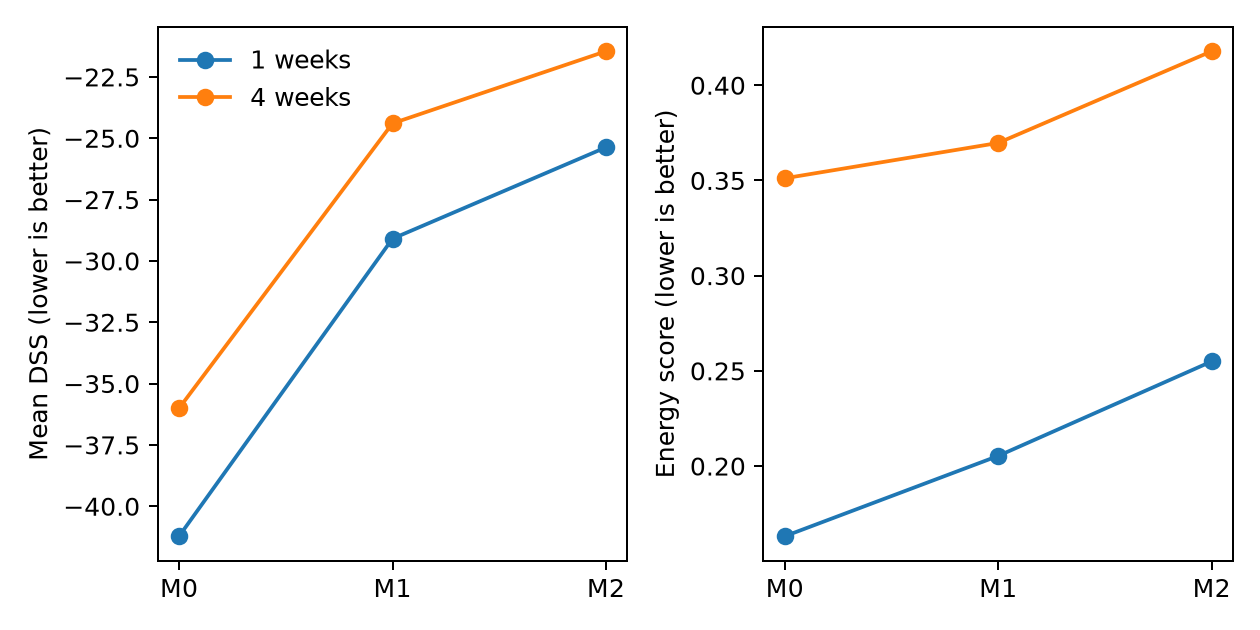
\includegraphics[width=0.95\linewidth,height=\textheight,keepaspectratio]{../figures/validated/scores.png}

}

\caption{\label{fig-scores}Mean--covariance and ensemble scores for the
accepted classical run. No Bayesian model is represented.}

\end{figure}%

\section{One-week results and maturity
dependence}\label{one-week-results-and-maturity-dependence}

Table~\ref{tbl-h1} reports the common-origin one-week forecasts. The
random walk again has the lowest aggregate DSS, Energy Score and pooled
RMSE among the accepted models. These results do not imply that a weekly
random walk will dominate at longer horizons, with different factors, or
after a corrected stochastic-volatility model is introduced.

\begin{longtable}[]{@{}lllllll@{}}
\caption{Accepted classical forecasts at 1-week horizon; 130 origins per
model. RMSE is pooled across origins and maturities; yields and width
are in percentage points.}\label{tbl-h1}\tabularnewline
\toprule\noalign{}
Model & DSS & Energy & RMSE & MAE & Coverage & Width \\
\midrule\noalign{}
\endfirsthead
\toprule\noalign{}
Model & DSS & Energy & RMSE & MAE & Coverage & Width \\
\midrule\noalign{}
\endhead
\bottomrule\noalign{}
\endlastfoot
M0 & -41.223 & 0.163 & 0.100 & 0.067 & 0.905 & 0.308 \\
M1 & -29.095 & 0.205 & 0.117 & 0.083 & 0.905 & 0.342 \\
M2 & -25.370 & 0.255 & 0.139 & 0.099 & 0.944 & 0.525 \\
\end{longtable}

Figure~\ref{fig-maturity} shows that the horizon-level mean hides
differences across maturities. A model can have reasonable marginal
coverage yet misrepresent joint dependence. Figure~\ref{fig-pit} pools
marginal PITs to visualize distributional shape, but pooling dependent
maturities does not create an enlarged independent time series. Formal
calibration tests would require a dependence-aware design and separate
treatment of maturity-specific hypotheses.

\begin{figure}

\centering{

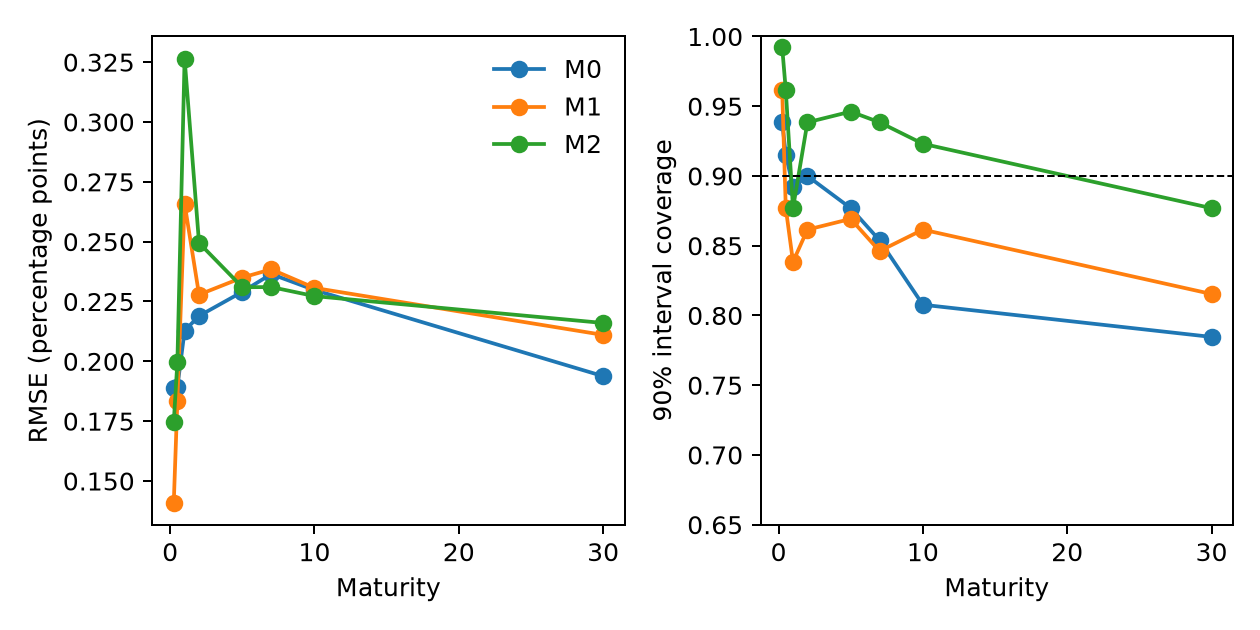
\includegraphics[width=0.95\linewidth,height=\textheight,keepaspectratio]{../figures/validated/maturity.png}

}

\caption{\label{fig-maturity}Four-week maturity-specific RMSE and
marginal interval coverage from accepted saved forecasts.}

\end{figure}%

\begin{figure}

\centering{

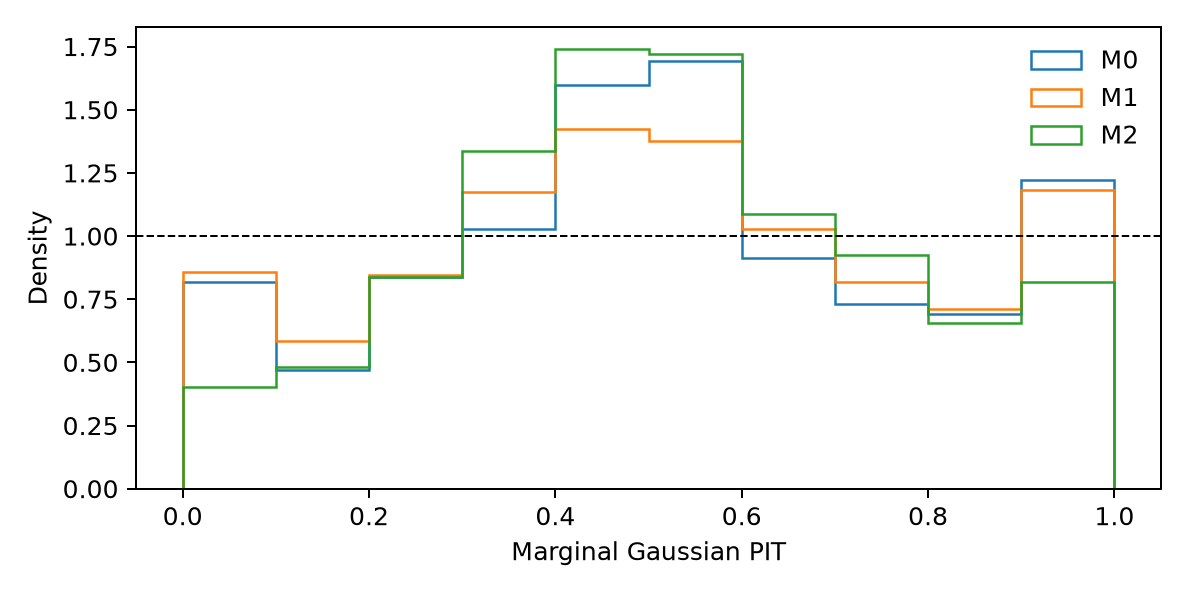
\includegraphics[width=0.95\linewidth,height=\textheight,keepaspectratio]{../figures/validated/pit.png}

}

\caption{\label{fig-pit}Pooled marginal Gaussian PIT histogram at four
weeks. Uniformity is a reference shape; no independent-observation test
is claimed.}

\end{figure}%

\section{Paired score uncertainty}\label{paired-score-uncertainty}

\begin{longtable}[]{@{}llllll@{}}
\caption{Descriptive paired loss differences with Bartlett HAC standard
errors (three origin lags). Normal intervals are approximate; no claim
about Bayesian volatility follows.}\label{tbl-comparison}\tabularnewline
\toprule\noalign{}
Horizon & Loss & M2 minus M0 & HAC SE & 95\% lower & 95\% upper \\
\midrule\noalign{}
\endfirsthead
\toprule\noalign{}
Horizon & Loss & M2 minus M0 & HAC SE & 95\% lower & 95\% upper \\
\midrule\noalign{}
\endhead
\bottomrule\noalign{}
\endlastfoot
1 & dss & 15.853 & 3.004 & 9.965 & 21.740 \\
1 & energy\_score & 0.092 & 0.012 & 0.069 & 0.114 \\
4 & dss & 14.553 & 1.902 & 10.826 & 18.280 \\
4 & energy\_score & 0.067 & 0.008 & 0.052 & 0.082 \\
\end{longtable}

Table~\ref{tbl-comparison} compares classical DNS with the random walk
using common-date loss differences. A positive value means DNS has the
larger loss. These comparisons are descriptive checks of the accepted
calculation. They do not replace the primary Model 4 versus Model 5
comparison and should not be repurposed as evidence that stochastic
volatility is unnecessary.

The finite sample contains different interest-rate environments, but
this draft does not assign regimes by inspecting which partitions
produce favorable significance. Formal regime splits, prior sensitivity
and covariance-floor sensitivity should be specified before their
results are used to refine the hypothesis. The Variogram Score is
included as an optional descriptive metric; it is not a substitute for
those missing experiments.

\section{Completed execution is not completed
inference}\label{completed-execution-is-not-completed-inference}

The six-model computation produced 1,560 records, finite arrays and
positive-definite covariances. It took 3,266.1 seconds. Its state-space
optimizer reported success on all 130 origins. Those are reproducible
execution facts, not accepted Bayesian scientific results.

The final-origin SV chains showed split \(\widehat R\) as high as 3.597
and a legacy ESS estimate as low as 5.324. Table~\ref{tbl-failed-diag}
gives the actual diagnostics. The mean-equation coefficients can mix
better than volatility persistence and intercept parameters; acceptable
diagnostics for one subset cannot validate the remainder. The ESS
implementation is approximate and is not the rank-normalized bulk/tail
procedure required for a modern posterior audit.

\begin{longtable}[]{@{}llll@{}}
\caption{Failed two-chain diagnostics at 28 November 2025 from the
quarantined run. ESS is an approximate legacy estimate, not
rank-normalized bulk/tail ESS.}\label{tbl-failed-diag}\tabularnewline
\toprule\noalign{}
Factor & Parameter & Split R-hat & ESS estimate \\
\midrule\noalign{}
\endfirsthead
\toprule\noalign{}
Factor & Parameter & Split R-hat & ESS estimate \\
\midrule\noalign{}
\endhead
\bottomrule\noalign{}
\endlastfoot
level & a & 1.010 & 609.998 \\
level & b & 1.010 & 569.776 \\
level & h\_intercept & 2.717 & 5.446 \\
level & phi & 2.795 & 5.324 \\
level & sigma2\_h & 1.511 & 10.640 \\
slope & a & 1.003 & 386.041 \\
slope & b & 1.000 & 380.677 \\
slope & h\_intercept & 3.421 & 6.311 \\
slope & phi & 3.597 & 6.037 \\
slope & sigma2\_h & 1.561 & 14.451 \\
curvature & a & 1.000 & 168.080 \\
curvature & b & 1.000 & 215.709 \\
curvature & h\_intercept & 1.627 & 18.778 \\
curvature & phi & 1.677 & 17.565 \\
curvature & sigma2\_h & 1.441 & 15.337 \\
\end{longtable}

An independent moment test found that the transcribed mixture implied a
log-innovation mean of approximately −0.6655, whereas the analytical
expectation of \(\log\chi^2_1\) is approximately −1.2704. This
discrepancy rejects the approximation before considering sophisticated
posterior diagnostics. Another regression test showed that the variance
update omitted its stationary initial-state contribution. These defects
and non-convergence preclude interpreting original favorable M5 scores
as evidence of better forecasting.

Other departures matter independently. The M4 and M5 coefficient priors
were not matched. M4 used direct posterior draws instead of specified
MCMC. M3's covariance propagation was incorrect. Conventional predictive
means were unnecessarily estimated from small simulated ensembles rather
than exact fitted means. Finally, original aggregated
\texttt{rmse\_curve} was a mean of curve-level RMSEs, not pooled RMSE.
The separate classical rerun resolves the latter two issues for M0--M2
and separates unaccepted models.

\section{Robustness achieved and still
required}\label{robustness-achieved-and-still-required}

Accepted artifacts pass checks for date uniqueness, common origins,
target boundaries, units, finite scenarios, covariance definiteness and
exact score reconstruction. An official-source slice matches supplied
raw data. Independent analytical tests verify classical factor moments
and Nelson--Siegel loadings. These are verification checks, not a full
economic robustness study.

Missing scientific robustness includes corrected multi-chain SV
estimation, matched prior sensitivity, multiple representative
diagnostic windows, state-space likelihood-start sensitivity, a
release-lag design, vintage sensitivity, reconstruction-covariance
alternatives, stronger ensemble stability checks and a validated MCS.
The sample and origin schedule have not been reduced to conceal
estimation failure. Rather, the scope of accepted results has been
narrowed explicitly.

\chapter{Fixed-income scenario illustration}\label{sec-risk}

\section{Risk object and
approximation}\label{risk-object-and-approximation}

For an equal-market-value basket with maturity weights \(w_i=1/8\), this
draft maps yield scenarios into a first-order duration-shock loss,

\begin{equation}\protect\phantomsection\label{eq-loss}{
\ell_{t,h}^{(m)}=\sum_{i=1}^8 w_i\tau_i\frac{Y_{i,t+h}^{(m)}-Y_{i,t}}{100}.
}\end{equation}

This is a local sensitivity illustration in units of initial basket
value. It is not a realized total-return backtest. It holds duration
exposure at the origin, ignores aging, coupon cash flows, financing,
convexity, rebalancing and transaction costs. The duration mapping is
not asserted exact under an unverified yield-compounding convention.
Presenting it as an investable bond portfolio return would overstate the
evidence.

VaR at confidence level \(\alpha\) is the empirical loss quantile, and
ES is the simulated mean loss above that quantile. At 99\% confidence,
an ensemble of 1,024 curves contains few tail observations, so ES is
noisy. The complete risk-scenario CSV retains both 95\% and 99\%
outputs, but the main table emphasizes the less sparse 95\%
illustration. More tail simulation and stability analysis are needed
before a risk-management conclusion.

\section{Illustration and backtesting
limits}\label{illustration-and-backtesting-limits}

\begin{longtable}[]{@{}lllll@{}}
\caption{Four-week first-order duration-shock risk for an
equal-market-value maturity basket. VaR/ES are percentages of initial
value, not total-return risk measures. UC tests are
exploratory.}\label{tbl-risk}\tabularnewline
\toprule\noalign{}
Model & Mean VaR95 & Mean ES95 & Exceptions & UC p \\
\midrule\noalign{}
\endfirsthead
\toprule\noalign{}
Model & Mean VaR95 & Mean ES95 & Exceptions & UC p \\
\midrule\noalign{}
\endhead
\bottomrule\noalign{}
\endlastfoot
M0 & 1.824 & 2.282 & 14 & 0.008 \\
M1 & 1.908 & 2.395 & 14 & 0.008 \\
M2 & 2.299 & 2.913 & 10 & 0.190 \\
\end{longtable}

Table~\ref{tbl-risk} uses only accepted classical distributions.
Exception counts are compared with nominal 5\% tail probability.
Reported unconditional-coverage p-values are exploratory asymptotic
diagnostics for the duration-shock target. A nonsignificant result would
not prove model adequacy, especially with only 130 origins and few tail
events.

Christoffersen-style transition diagnostics exist in the legacy code,
but their adequacy at sparse exception counts and under this risk
definition has not been independently established. No accepted
ES-specific backtest is provided. Computing a simulated ES is not
equivalent to testing ES forecasts. Bayesian scenario VaR/ES and formal
comparative risk backtests remain pending because their predictive
distributions are not accepted.

\chapter{Conclusions and outstanding research}\label{sec-conclusions}

\section{What available evidence
establishes}\label{what-available-evidence-establishes}

For the specified Canadian historical panel and 130 common evaluation
origins, the separately verified random-walk benchmark outperforms
PCA--VAR and two-step Gaussian DNS on average DSS, Energy Score and
pooled RMSE at both tested horizons. At four weeks, its mean DSS is
−36.006 and pooled RMSE is 0.213 percentage points. Marginal interval
coverage is below nominal, so forecast accuracy should not be confused
with complete calibration.

The principal Bayesian research question remains unanswered. A six-model
process completed, but defective stochastic-volatility inference and
unmatched priors invalidate the controlled comparison. The scientific
response is to retain failure evidence, correct the implementation, test
it independently and rerun the Bayesian pair only after a representative
pilot passes acceptance gates. It is not to select favorable scores or
describe non-converged posterior draws as established uncertainty
estimates.

\section{Work required before a complete
paper}\label{work-required-before-a-complete-paper}

The exact no-leverage mixture must be verified against its source and
full conditional updates must agree with the documented prior and
initial-state treatment. The constant-volatility and
stochastic-volatility models need matched coefficient priors and a clear
account of rolling estimation. Independent chains must be assessed at
early, middle and late windows with reliable diagnostics and
score-stability checks. M3 requires a corrected and independently
checked forecast covariance and likelihood fit.

A full paper additionally needs remaining literature-access gaps
resolved where possible, a release-time interpretation or explicitly
revised real-time design, validated multiple-model inference and risk
backtests appropriate to an actual portfolio definition. The official
guidelines require the student's own understanding, review and prior
discussion of AI use with the supervisor. No automated statement can
establish that approval.

This first draft is a reproducible, reviewable partial artifact rather
than a completed research finding. Its main methodological lesson is
specific: an expanded volatility model does not earn credibility from
execution success alone. Verification of the likelihood approximation,
posterior exploration, forecast information set and scoring calculations
is integral to answering the economic question.

\chapter{Analytical derivations and numerical
checks}\label{sec-appendix}

\section{Least-squares factor
extraction}\label{least-squares-factor-extraction}

For fixed \(\lambda\), minimize \(g(f)=(Y-\Lambda f)'(Y-\Lambda f)\).
Differentiation gives
\(\partial g/\partial f=-2\Lambda'Y+2\Lambda'\Lambda f\). Setting the
derivative to zero yields Equation~\ref{eq-extraction} when the three
columns have full rank. Least squares avoids explicitly computing an
inverse, which would be less stable if loadings were poorly conditioned.

As \(x=\lambda\tau\) approaches zero, \((1-e^{-x})/x\) approaches one.
The implementation uses \texttt{expm1} to avoid cancellation for small
positive \(x\). Curvature approaches zero at the short end. At long
maturities both nonlevel loadings approach zero. These limits establish
interpretation and basic sign checks; they do not identify factors
econometrically without further assumptions.

\section{AR and VAR forecast moments}\label{ar-and-var-forecast-moments}

Repeated substitution gives
\(f_{t+h}=b^hf_t+a\sum_{k=0}^{h-1}b^k+\sum_{k=0}^{h-1}b^k\eta_{t+h-k}\).
Taking expectations yields the mean in Equation~\ref{eq-ar-moments}.
Independent zero-mean innovations eliminate cross terms, giving
\(q\sum b^{2k}\) for its variance. The finite-sum form remains well
defined when a fitted slope is near one.

The matrix version replaces \(b^k\) with \(A^k\) and yields
Equation~\ref{eq-var-forecast}. If the origin state has filtered
covariance \(P_t\), an additional term \(A^hP_t(A^h)'\) appears. This
explains why applying \(A^{2h}\) on both sides, as in original M3 code,
is wrong: it multiplies diagonal uncertainty by fourth rather than
second powers of the horizon transition.

\section{Yield predictive covariance}\label{yield-predictive-covariance}

For a fixed loading matrix and independent observation noise,
\(\operatorname{Var}(Y\mid\mathcal I_t)=\Lambda\operatorname{Var}(f\mid\mathcal I_t)\Lambda'+R_t\).
Reconstruction uncertainty is added once at the future observation, not
at every transition. In a Bayesian model, factor variance must include
both conditional innovation uncertainty and dispersion in conditional
means across posterior draws.

Estimating an eight-dimensional covariance from a small ensemble can add
noise in low-variance directions. Analytic addition of \(R_t\) to a
factor-level posterior covariance is a useful stability check, but
changing the estimator must be documented consistently. The accepted
classical run avoids this issue through exact fitted moments.

\section{Stationary stochastic-volatility
update}\label{stationary-stochastic-volatility-update}

Write \(h_t=c+\phi h_{t-1}+u_t\) with \(c=(1-\phi)\omega\). Under
stationarity, \(h_1\sim N(c/(1-\phi),q/(1-\phi^2))\), where
\(q=\sigma_u^2\). For an inverse-gamma prior of shape \(a_0\) and scale
\(b_0\), the full conditional has

\begin{equation}\protect\phantomsection\label{eq-sv-update}{
a_n=a_0+\frac n2,\qquad
b_n=b_0+\frac12\left[\sum_{t=2}^n(h_t-c-\phi h_{t-1})^2
 +(1-\phi^2)\left(h_1-\frac{c}{1-\phi}\right)^2\right].
}\end{equation}

The initial-state term and degree-of-freedom contribution are required
if the remaining sampler uses a stationary initial density. Original
code omitted the contribution even though a correct helper existed. A
regression test now checks that the sampler uses that helper. This
repair is necessary, not sufficient, for acceptance.

For standard normal \(z\), the analytical mean of \(\log z^2\) is
\(\psi(1/2)+\log 2\), and variance is \(\psi_1(1/2)\). These are direct
checks for a Gaussian approximation to the log-square distribution.
Moment agreement is not a full density-accuracy test, but the original
mixture failed even the mean check.

\section{Score reconstruction and data
integrity}\label{score-reconstruction-and-data-integrity}

The accepted archive contains 780 distinct forecast keys. Recomputing
DSS from every saved mean, covariance and target reproduces the score
CSV up to roundoff; maximum absolute discrepancy is approximately
\(2.84\times10^{-14}\). The minimum covariance eigenvalue is positive.
These checks address consistency between predictions and reporting, not
the truth of assumptions.

The processor previously wrote test-fixture provenance into the global
source manifest, contaminating it with a temporary three-row example. A
failing isolation test established the cause; manifests are now written
next to their own outputs. The real panel and manifest were rebuilt.
Tests use the approved scratch directory and do not overwrite raw
sources.

\chapter*{Supplementary maturity
results}\label{supplementary-maturity-results}
\addcontentsline{toc}{chapter}{Supplementary maturity results}

\begin{longtable}[]{@{}llll@{}}
\caption{Four-week point accuracy and marginal 90\% interval
coverage.}\label{tbl-maturity}\tabularnewline
\toprule\noalign{}
Model & Maturity & RMSE & Coverage \\
\midrule\noalign{}
\endfirsthead
\toprule\noalign{}
Model & Maturity & RMSE & Coverage \\
\midrule\noalign{}
\endhead
\bottomrule\noalign{}
\endlastfoot
M0 & 0.250 & 0.189 & 0.938 \\
M0 & 0.500 & 0.189 & 0.915 \\
M0 & 1.000 & 0.213 & 0.892 \\
M0 & 2.000 & 0.219 & 0.900 \\
M0 & 5.000 & 0.229 & 0.877 \\
M0 & 7.000 & 0.236 & 0.854 \\
M0 & 10.000 & 0.230 & 0.808 \\
M0 & 30.000 & 0.194 & 0.785 \\
M1 & 0.250 & 0.141 & 0.962 \\
M1 & 0.500 & 0.183 & 0.877 \\
M1 & 1.000 & 0.266 & 0.838 \\
M1 & 2.000 & 0.228 & 0.862 \\
M1 & 5.000 & 0.235 & 0.869 \\
M1 & 7.000 & 0.238 & 0.846 \\
M1 & 10.000 & 0.231 & 0.862 \\
M1 & 30.000 & 0.211 & 0.815 \\
M2 & 0.250 & 0.175 & 0.992 \\
M2 & 0.500 & 0.200 & 0.962 \\
M2 & 1.000 & 0.326 & 0.877 \\
M2 & 2.000 & 0.249 & 0.938 \\
M2 & 5.000 & 0.231 & 0.946 \\
M2 & 7.000 & 0.231 & 0.938 \\
M2 & 10.000 & 0.227 & 0.923 \\
M2 & 30.000 & 0.216 & 0.877 \\
\end{longtable}

The table retains each maturity rather than treating a curve-level
average as a complete description. Additional calibration by confidence
level, subperiod and origin remains future work. Saved arrays make
extensions reproducible without refitting accepted benchmarks, but
post-hoc summaries must be identified as such.

\chapter*{Bibliography}\label{bibliography}
\addcontentsline{toc}{chapter}{Bibliography}

\protect\phantomsection\label{refs}
\begin{CSLReferences}{1}{0}
\bibitem[\citeproctext]{ref-bocdata}
Bank of Canada. (2026). \emph{Yield curves for zero-coupon bonds}.
\url{https://www.bankofcanada.ca/rates/interest-rates/bond-yield-curves/}

\bibitem[\citeproctext]{ref-bolder2004canadian}
Bolder, D. J., Johnson, G., \& Metzler, A. (2004). \emph{An empirical
analysis of the canadian term structure of zero-coupon interest rates}
(Nos. 2004-48). Bank of Canada.
\url{https://publications.gc.ca/site/eng/9.559261/publication.html}

\bibitem[\citeproctext]{ref-caldeira2010bayesian}
Caldeira, J. F., Laurini, M. P., \& Portugal, M. S. (2010). Bayesian
inference applied to dynamic nelson-siegel model with stochastic
volatility. \emph{Brazilian Review of Econometrics}, \emph{30}(1),
123--161. \url{https://doi.org/10.12660/bre.v30n12010.3502}

\bibitem[\citeproctext]{ref-dawid1999coherent}
Dawid, A. P., \& Sebastiani, P. (1999). Coherent dispersion criteria for
optimal experimental design. \emph{The Annals of Statistics},
\emph{27}(1), 65--81. \url{https://doi.org/10.1214/aos/1018031101}

\bibitem[\citeproctext]{ref-diebold2006forecasting}
Diebold, F. X., \& Li, C. (2006). Forecasting the term structure of
government bond yields. \emph{Journal of Econometrics}, \emph{130}(2),
337--364. \url{https://doi.org/10.1016/j.jeconom.2005.03.005}

\bibitem[\citeproctext]{ref-diebold2006macroeconomy}
Diebold, F. X., Rudebusch, G. D., \& Aruoba, S. B. (2006). The
macroeconomy and the yield curve: A dynamic latent factor approach.
\emph{Journal of Econometrics}, \emph{131}(1-2), 309--338.
\url{https://doi.org/10.1016/j.jeconom.2005.01.011}

\bibitem[\citeproctext]{ref-gneiting2007strictly}
Gneiting, T., \& Raftery, A. E. (2007). Strictly proper scoring rules,
prediction, and estimation. \emph{Journal of the American Statistical
Association}, \emph{102}(477), 359--378.
\url{https://doi.org/10.1198/016214506000001437}

\bibitem[\citeproctext]{ref-hansen2011model}
Hansen, P. R., Lunde, A., \& Nason, J. M. (2011). The model confidence
set. \emph{Econometrica}, \emph{79}(2), 453--497.
\url{https://doi.org/10.3982/ecta5771}

\bibitem[\citeproctext]{ref-hautsch2012bayesian}
Hautsch, N., \& Yang, F. (2012). Bayesian inference in a stochastic
volatility nelson--siegel model. \emph{Computational Statistics \& Data
Analysis}, \emph{56}(11), 3774--3792.
\url{https://doi.org/10.1016/j.csda.2010.07.003}

\bibitem[\citeproctext]{ref-omori2007stochastic}
Omori, Y., Chib, S., Shephard, N., \& Nakajima, J. (2007). Stochastic
volatility with leverage: Fast and efficient likelihood inference.
\emph{Journal of Econometrics}, \emph{140}(2), 425--449.
\url{https://doi.org/10.1016/j.jeconom.2006.07.008}

\bibitem[\citeproctext]{ref-patton2011volatility}
Patton, A. J. (2011). Volatility forecast comparison using imperfect
volatility proxies. \emph{Journal of Econometrics}, \emph{160}(1),
246--256. \url{https://doi.org/10.1016/j.jeconom.2010.03.034}

\bibitem[\citeproctext]{ref-sarkisian2024bayesian}
Sarkisian, D. (2024). \emph{A bayesian approach to yield curve modelling
and forecasting with stochastic volatility for interest rate risk
management} {[}Master's thesis, Delft University of Technology{]}.
\url{https://resolver.tudelft.nl/uuid:8510487e-d59f-4a89-93dd-dc685cd06bb6}

\bibitem[\citeproctext]{ref-scheuerer2015variogram}
Scheuerer, M., \& Hamill, T. M. (2015). Variogram-based proper scoring
rules for probabilistic forecasts of multivariate quantities.
\emph{Monthly Weather Review}, \emph{143}(4), 1321--1334.
\url{https://doi.org/10.1175/mwr-d-14-00269.1}

\end{CSLReferences}




\end{document}
